\documentclass[border=2pt]{standalone}
\usepackage{tikz}
\usetikzlibrary{positioning}
\begin{document}
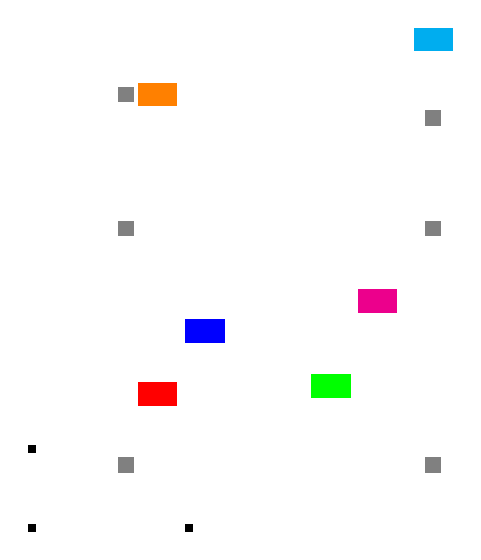
\begin{tikzpicture}[on grid,
  base/.style={fill=gray,minimum width=2mm,minimum height=2mm,inner sep=0pt,outer sep=0pt},
  probe/.style={minimum width=5mm,minimum height=3mm,inner sep=0pt,outer sep=0pt}]
  \fill (-.5mm,-.5mm) rectangle (.5mm,.5mm);
  \fill (19.5mm,-.5mm) rectangle (20.5mm,.5mm);
  \fill (-.5mm,9.5mm) rectangle (.5mm,10.5mm);
  \begin{scope}[x={(13mm,4mm)},y={(-3mm,9mm)}]
    % Explicit physical source coordinates isolate the positioning shifts.
    \node[base] (a) at (12mm,8mm) {};
    \node[base] (b) at (51mm,8mm) {};
    \node[base] (c) at (12mm,38mm) {};
    \node[base] (d) at (51mm,38mm) {};
    \node[base] (e) at (12mm,55mm) {};
    \node[base] (f) at (51mm,52mm) {};
    \node[probe,fill=red,above right=1 and 7mm of a] {};
    \node[probe,fill=green,above left=6mm and 1 of b] {};
    \node[probe,fill=blue,below right=1 and 1 of c] {};
    \node[probe,fill=magenta,below left=1 of d] {};
    \node[probe,fill=orange,right=1 and 7mm of e] {};
    \node[probe,fill=cyan,above=6mm and 1 of f] {};
  \end{scope}
\end{tikzpicture}
\end{document}
